\section{Deconvolution}
\subsection{Inverse filter}
The first and most obvious type of deconvolution is using an inverse filter. We have a blurred image $g$, we found an estimation of the psf ($h_e$) in the previous section %TODO ça sera tjs des sections ?
. So we are theoretically ready to find the original image. We had
\begin{equation}
 g =  h*f,
\end{equation}
in frequency domain
\begin{equation}
G = HF. 
\end{equation}

Using $H_e$, the estimated psf in frequency domain, we can get $F_e$ an so $f_e$ by 
\begin{equation}
F_{e} = H_{e}^{-1} G
\end{equation} 

However it's clear that if we add some noise this model doesn't work anymore. Indeed as shown on figure \ref{fig:psfFFT}, $H_e$ has some value near zero, especially at high frequencies because a blur typically reduces these frequencies. So when we divide $G$ by $H_e$, the noise is strongly amplified by the value near zero. This problem explains the results obtained on figure XXX.   

\begin{figure}
\centering
%\missingfigure{T'as oublié de la pusher}
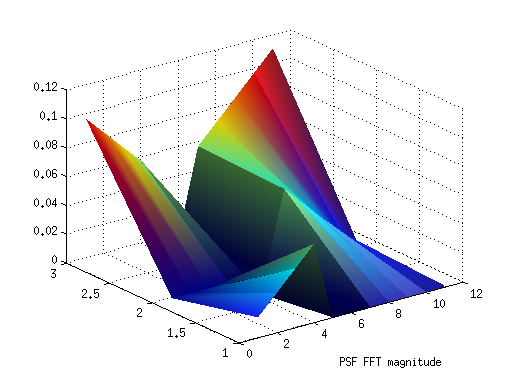
\includegraphics[scale=0.5]{../Images/psfFFT.png}
\caption{FFT of the psf}
\label{fig:psfFFT}
\end{figure}

\begin{myfig}{cameraman_F_diff}
  {Effect of the noise with an inverser filter.}
  \mysubfig{matb-nonoise}{$S$ for the cameraman.}{0.32}
  \mysubfig{cameraman_F}{$S$ for the cameraman.}{0.32}
  \mysubfig{matb-noisy}{$S$ for the cameraman with a blur of $(40, 30)$ with ``replicate''.}{0.32}
  \mysubfig{cameraman_F_circular_40-30}{$S$ for the cameraman with a blur of $(40, 30)$ with ``circular''.}{0.32}
\end{myfig}


\subsection{Lucy-Richarson}
\label{subsec:Lucy}
\subsubsection{Theory behind the method}
The method was introduced in~\cite{richardson1972bayesian} and
then in~\cite{lucy1974iterative} by Richarson and Lucy respectively.
I these articles, $f$ and $g$ are considered as probability function.
\cite{richardson1972bayesian} says (translated in our notations)
``Units of enery (which may be considered as unique events)
originating at a point in $f$ are distributed at points in $g$
according to the frequencies indicated by $h$''.
However, the justification of~\cite{richardson1972bayesian} (in 1D) uses
$P(f(x)) = \frac{f(x)}{\sum_x f(x)}$ which does not seem
very appropriate.

When \cite{richardson1972bayesian} talks about energy,
that refers to the light which is quantized with photons.
That quantization gives us a reason to model the noise with
poisson distribution.
This modelization of the noise is called the shot noise and
is developped in~\cite{blanter2000shot}.
This model of the noise is used by~\cite{hebert1989generalized}.
\cite{temerinac2010tile} base on~\cite{hebert1989generalized}
and this model of the noise to show (even in 3D)
that the Lucy-Richardson algorithm gives the MLE of $f$ of this
model.

They suggest that $G \sim \pois(h * f)$ ($G$ is capitilize sinced it is a random function).
Therefore,
\begin{align*}
  L(f) & = P(g|f)\\
  & = \prod_{(x,y)} \frac{[(h*f)(x,y)]^{g(x,y)} \exp(-(h*f)(x,y))}{(g(x,y))!}\\
  l(f) & = \sum_{(x,y)} g(x,y)\log((h*f)(x,y)) - (h*f)(x,y) -\log(g(x,y)!).
\end{align*}
Let's first develop
\begin{align*}
  \fpart{(h*g)(x,y)}{f(a,b)} & = \fpart{}{f(a,b)}\sum_{(i,j)}f(i,j)h(x-i,y-j)\\
  \fpart{(h*g)(x,y)}{f(a,b)} & = h(x-a,y-b).
\end{align*}
Consequently, we have
\begin{align*}
  \fpart{l(f)}{f(a,b)} & = \sum_{(x,y)} \left(\frac{g(x,y)}{(h*f)(x,y)} - 1\right) \fpart{(h*g)(x,y)}{f(a,b)}\\
  & = \sum_{(x,y)} \left(\frac{g(x,y)}{(h*f)(x,y)} - 1\right) h(x-a,y-b)\\
  & = \left(\left(\frac{g(x,y)}{(h*f)(x,y)} - 1\right) * h(-x,-y)\right)(a,b)\\
  & = \left(\left(\frac{g(x,y)}{(h*f)(x,y)}\right) * h(-x,-y)\right)(a,b) - 1 * h(-x,-y)\\
  & = \left(\left(\frac{g(x,y)}{(h*f)(x,y)}\right) * h(-x,-y)\right)(a,b) - \left(\sum_{(i,j)} h(-x-i,-y-j)\right)(a,b).
\end{align*}
As explained in the mathematical model,
\[ \sum_{(i,j)} h(i,j) = 1 \]
so we have
\[ \nabla l(f) = \frac{g(x,y)}{(h*f)(x,y)} * h(-x,-y) - 1. \]
To get the minimum of $l(f)$, $\nabla l(f)$ needs to be 0.
Therefore
\begin{equation}
  \label{eq:lucy-cond}
  \frac{g(x,y)}{(h*\hat{f})(x,y)} * h(-x,-y) = 1.
\end{equation}
If we multiply each side by $f(x,y)$, we get
\[ f(x,y)\left(\frac{g(x,y)}{(h*\hat{f})(x,y)} * h(-x,-y)\right) = f(x,y) \]
which can be solved iteratively using the fixed point method which gives us
\[ f_{k+1}(x,y) = f_k(x,y)\left(\frac{g(x,y)}{(h*f_k)(x,y)} * h(-x,-y)\right). \]

If we converge to $f$, we know that $\nabla l(f) = 0$
so $f$ is a critical point of $l(f)$.
However, we can't say that it maximize $l$ even
if we proof that the hessian is negatively definite since
the solution of the equation~\eqref{eq:lucy-cond}
is not unique.

For example, in 1-D, if
\begin{align*}
  h & = \frac{1}{2}
  \begin{pmatrix}
    1 & 1
  \end{pmatrix},\\
  g & =
  \begin{pmatrix}
    \cdots & 1 & 1 & 1 & \cdots
  \end{pmatrix},
\end{align*}
we have the two following solutions
\begin{align*}
  f_1 & = \frac{1}{2}
  \begin{pmatrix}
    \cdots & 1 & 1 & 1 & 1 & \cdots
  \end{pmatrix},\\
  f_2 & =
  \begin{pmatrix}
    \cdots & 0 & 2 & 0 & 2 & \cdots
  \end{pmatrix}.
\end{align*}
However, since $h * f_1 = h * f_2 = g$ so they maybe both maximize $l$.
%For example, in 1-D, if
%\begin{align*}
%  h & = \frac{1}{2}
%  \begin{pmatrix}
%    1 & 1
%  \end{pmatrix},\\
%  g & =
%  \begin{pmatrix}
%    \cdots & 1 & \frac{3}{2} & 1 & \frac{3}{2} & \cdots
%  \end{pmatrix},
%\end{align*}
%we have the two following solutions
%\begin{align*}
%  f_1 & = \frac{1}{2}
%  \begin{pmatrix}
%    \cdots & \frac{1}{2} & \frac{3}{2} & \frac{3}{2} & \frac{1}{2} & \frac{5}{2} & \cdots
%  \end{pmatrix},\\
%  f_2 & =
%  \begin{pmatrix}
%    \cdots & 3 & 1 & 2 & 2 & 1 & 3 & 1 & 2 & 2 & 1 & \cdots
%  \end{pmatrix}.
%\end{align*}

\subsubsection{Intuitive understanding}
A big advantage with this method is that we can understand
it intuitively.
Let's analyse an iteration.
\begin{enumerate}
  \item We start with an estimate $f_k$ and we compute
    $h * f_k$ which would be $g$ if $f_k = f$.
  \item We then compute, for each pixel, the ratio between
    the expected value $g(x,y)$ and what we currently have
    (i.e.  $(h * g)(x,y)$).
    Let's call it $r(x,y)$.
  \item If $h$ was $\delta(x,y)$, we could just take
    $f_{k+1} = f_k \cdot r$ and we would be done in one
    iteration.
    But here $g(x,y)$ is not only influenced by
    $f(x,y)$ but also by neighbouring values of $f$.
  \item The idea is therefore to spread $r$ on the values
    that have influenced $g(x,y)$.
    And $r(x,y)$ will influence a pixel in $f_k$ with the same
    weight that it influence $g(x,y)$.
    That's why we convolve $r$ with $h(-x,-y)$.
  \item Since each pixel has a sum of weight of 1,
    it will be influenced by a weight of 1 of elements of $r$.
    The ratio in $r(x,y) * h(-x, -y)$ is then multiplied to
    $f_k(x,y)$ to get $f_{k+1}(x,y)$.
\end{enumerate}
\[ f_{k+1}(x,y) = f_k(x,y)\left(\frac{g(x,y)}{(h*f_k)(x,y)} * h(-x,-y)\right). \]

\subsubsection{Practical case}
For the train case, $f$ and $g$ are given in a finite rectangle
and they have the same size which causes problems on their borders.
To compute $h * f$ on the border of $f$ we do not have enough
information. The same problem appears when we need to
convolve with $h(-x,-y)$.

Let's take an example with a 1-D blur to the right
2 pixels long. The first index is 1 and the last is $n$.
\begin{itemize}
  \item For the convolution with $h(-x,-y)$,
    we have a problem with $f(n)$ because it influences
    $g(n)$ and $g(n+1)$ and since $g(n+1)$ is unknown.
    A solution would be to only listen to the feedback given
    by $g(n)$ but the sum of the weight of the feedbacks
    will not be 1.
    Consequently, we need to modify the method.
    We will not spread $r$ but $r-1$ and then do $+1$
    after the convolution with $h(-x)$ which gives (in 2-D)
    \begin{equation}
      \label{eq:lucy_iter_modif}
      f_{k+1}(x,y) = f_k(x,y)\left(1+\left(\frac{g(x,y)}{(h*f_k)(x,y)}-1\right) * h(-x,-y)\right).
    \end{equation}
    That way, $f(n)$ is influenced by $g(n)$ the same
    way it influence $g(n)$ which seems mandatory and
    the effet of $g(n+1)$ is the same as if
    $g(n+1) = (h*f)(n+1)$.
  \item For $h * f$,
    let's assume that we have a 1-D blur to the right of 2 pixels
    (index starting at 1).
    $(h*f)(1)$ depends on both $f(1)$ and $f(0)$ but $f(0)$ is not processed.
    \begin{enumerate}
      \item An first idea would be to make $f$ starts at 2.
        We would approximate $\hat{f}(1)$ with $g(1)$.
        $g(2)$ will be influence by $f(2)$ which is being estimated
        and $\hat{f}(1)$ which is considered to be known.
        The only difference will be that we do not update $\hat{f}(1)$
        each iteration.
        To get an better estimate for $\hat{f}(1)$, we can take
        $g(1+L/2)$ where $L$ is the length of the blur since
        that is the mean of the $L/2$ neighbours on the right and left
        of $g(1)$.
      \item A second idea would be to estimate $f$ from 0
        it would only be influenced by $g(1)$.
        We would therefore use equation~\eqref{eq:lucy_iter_modif}
        for the iteration for the reasons explained earlier.
        For the general case, we add pior values of $f$ to the
        estimation process until $2-L$.
    \end{enumerate}
\end{itemize}

For $f_0$ we usually start with a gray image (unicolor) which gives acceptable results.
That way,
\begin{align*}
  f_1(x,y) & = f_0(x,y)\left(\frac{g(x,y)}{(h*f_0)(x,y)} * h(-x,-y)\right)\\
               & = F_0\left(\frac{g(x,y)}{F_0} * h(-x,-y)\right)\\
               & = g(x,y) * h(-x,-y).
\end{align*}
which is already correct if $g$ is unicolor.

\subsection{Wiener}
\label{subsec:Wiener}
 Another deconvolution is the wiener one. The wiener filter is more robust than the inverse filter because it doesn't ignore the noise. We have in the frequency domain
\begin{equation}
G = HF + N,
\label{eq:FeHF}
\end{equation} 
 where $N$ is the DF transform of a noise $n$ with mean $0$, and we want to estimate $F_e$ based on the image observed $F$ and a filter $L$, i.e. 
 \begin{equation}
 F_e = LF.
 \label{eq:feLF}
 \end{equation}

To choose the filter $L$, we minimize 
\begin{equation}
\min \mathbb{E}\{|F - F_e|^2\},
\label{eq:FFe}
\end{equation}
and so, using equations \eqref{eq:FeHF} and \eqref{eq:feLF} we can transform equation \eqref{eq:FFe} in 
\begin{align}
\mathbb{E}\{|F - F_e|^2\} &= \mathbb{E}\{|F - L(HF+N)|^2\}\\
	&= \mathbb{E}\{|(1-LH)F - LN|^2\}
\end{align}

Then, let's introduce some notations concerning the power spectrum :
\begin{align}
S_f &= \mathbb{E}\{|F|^2\}\\
S_n &= \mathbb{E}\{|N|^2\}\\
\end{align}

After some computation and taking the derivative, we get

\begin{equation}
L = \frac{H^*+S_f}{|H|^2 S_f + S_n}.
\label{eq:LsemiFinal}
\end{equation}

Defining $NSR = \frac{S_n}{S_f}$, we can rewrite $L$ as 
\begin{equation}
L = \frac{H^*}{|H|^2 + NSR}.
\end{equation}

However, this filter needs an estimation of the noise and image variances, which are difficult to estimate. For further details on this estimation, please refer to the section \ref{sec:NSREstimation}.

\subsection{Regularisation}
\label{subsec:Reg}
%TODO
The last deconvolution method is the deconvolution using regularized filter. 
Instead of a simple inverse filter, we want to minimize the sum of two terms. The first one is the square of the error between the blurred image received and the blurred one using the psf and the original image we are looking for. The second term is used to smooth the image to a certain extent. The term $l(m,n)$ is chosen as a high pass filter in order to minimize the high-frequencies, i.e. the roughness in the solution. The parameter $\alpha$ controls the degree of roughness penalty. The higher the coefficient is, the smoother the image will be. %TODO source mathworks t

\begin{equation}
\sum_{m,n} \left[ (g(m,n) - h(m,n)*f(m,n))^2 + \alpha (l(m,n)*f(m,n))^2 \right]
\end{equation}

The using the Fourier transform, we get
\begin{equation}
\sum_{k,l} \{ [G(k,l) - H(k,l)F(k,l)]^2 + \alpha [L(k,l)F(k,l)]^2\}
\end{equation}

With the derivative we obtain
\begin{equation}
\hat{F_e}(k,l) = \frac{H(k,l)}{|H(k,l)|^2 + \alpha |L(k,l)|^2} G(k,l)
\end{equation}
So when the value of $H_e$ is near zero, the term $\alpha |L(k,l)|^2$ is there to avoid a too small denominator. 

